\documentclass[]{article}
\usepackage{graphicx}

\begin{document}

\title{Analyzing the Number of Updates Sent}
\maketitle
\newpage
The topology used is shown below. \\
\linebreak

\begin{center}
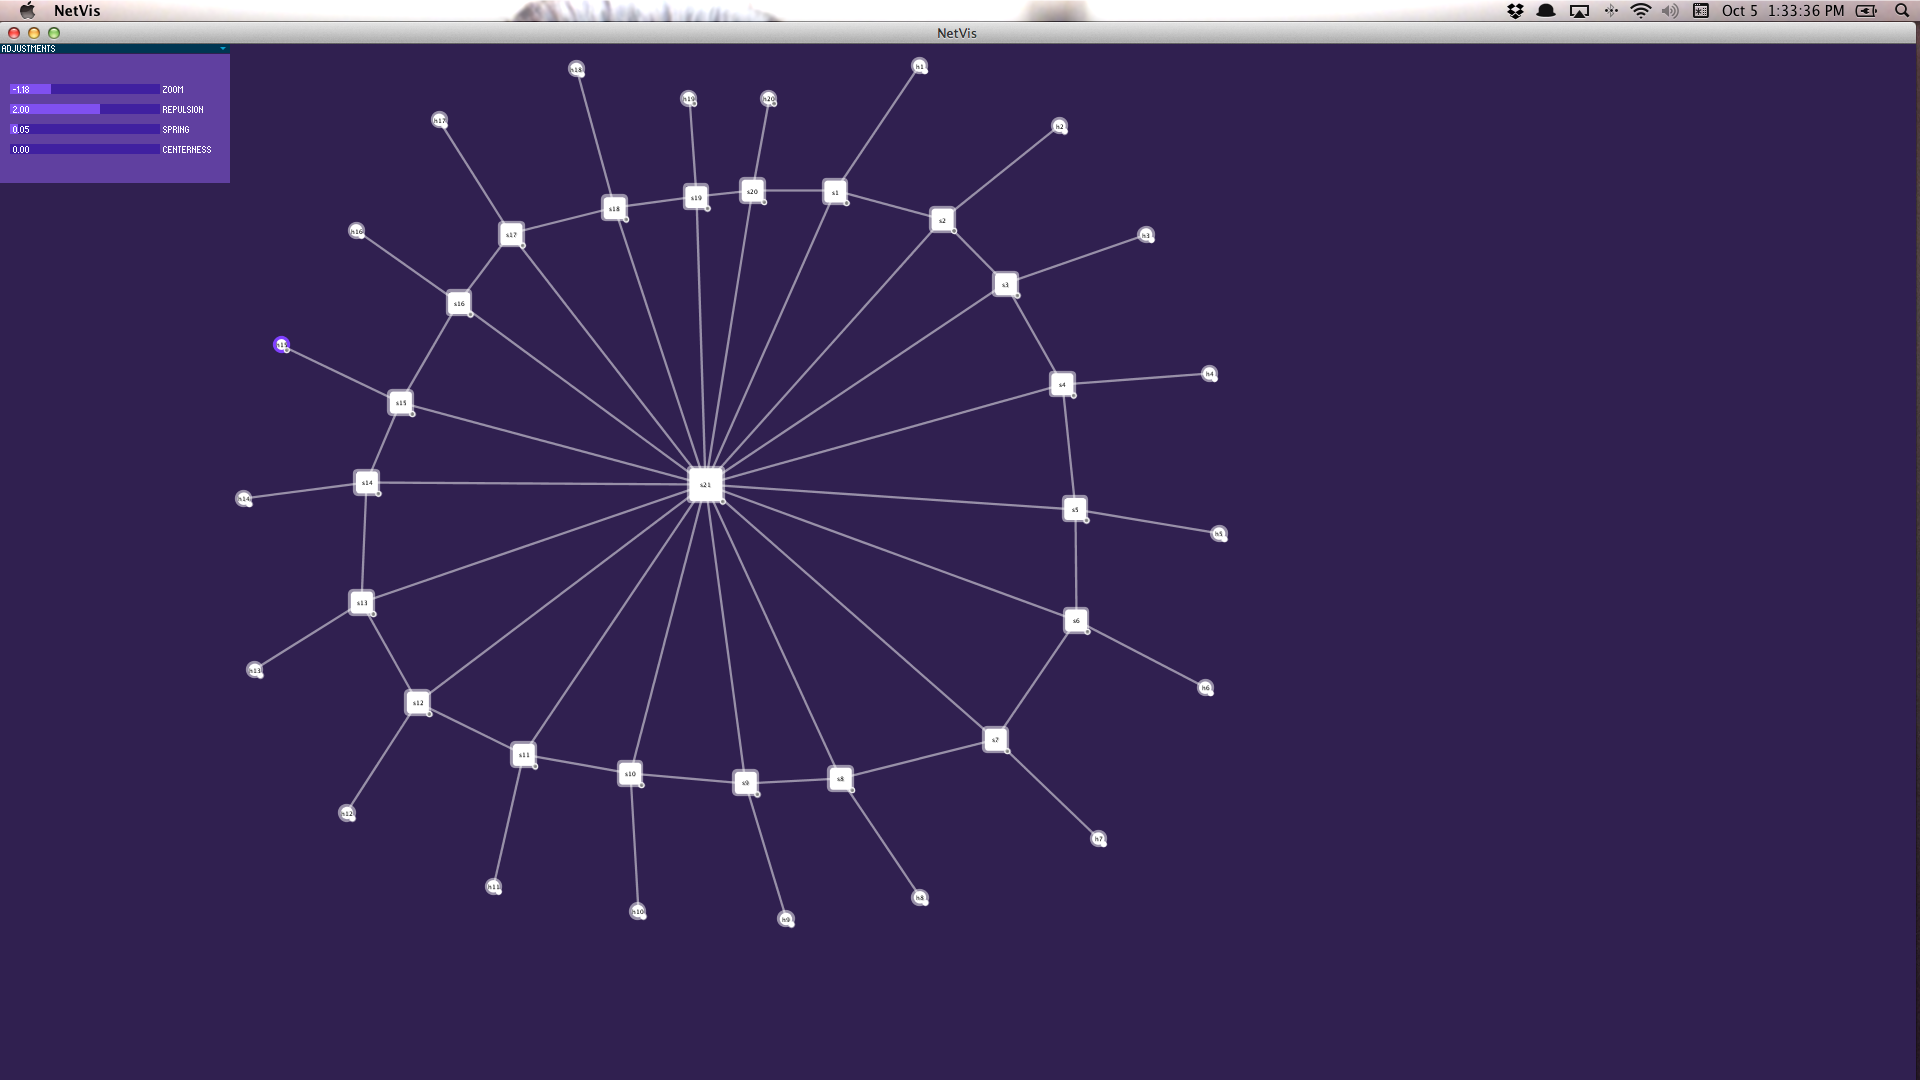
\includegraphics[width=10cm]{topology.png}
\linebreak
The total number of updates sent as a function of the number of routers in the topology is contained in the array: 

[51, 92, 145, 219, 299, 391, 495, 611, 739, 879, 1031, 1195, 1371, 1559, 1759, 1971, 2195, 2431, 2679, 2939, 3211, 3495, 3791, 4099, 4419, 4751, 5095, 5451, 5819, 6199, 6591, 6995, 7411, 7839, 8279, 8731, 9195, 9671, 10159, 10659, 11171, 11695, 12231, 12779, 13339, 13911, 14495, 15091]
\linebreak

The plot of this data is shown below.
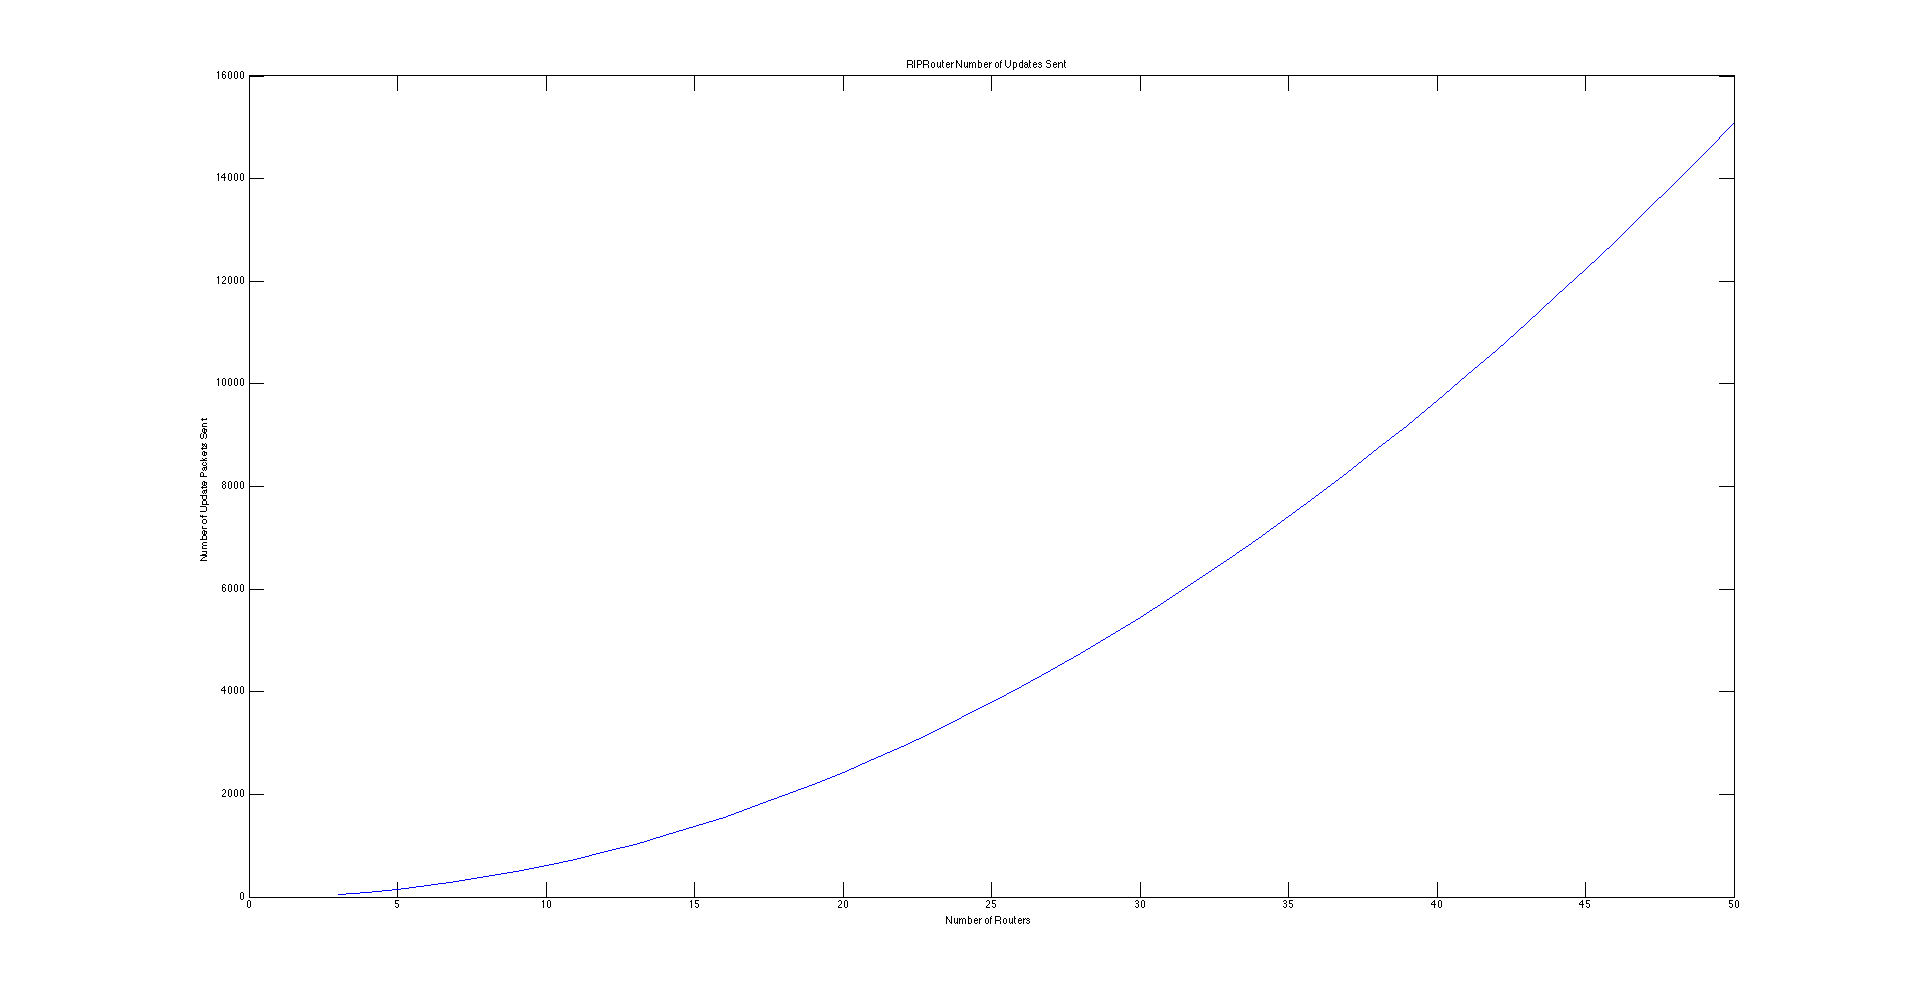
\includegraphics[width=13cm]{plot.png}
\end{center}
\end{document}